\documentclass{article}

\usepackage{url} 

\usepackage{pdfpages}
\usepackage{lastpage}
\usepackage{fancyhdr}
\usepackage{ngerman}

\usepackage{xcolor}
\usepackage{listings}
\usepackage{courier}

\usepackage{chngcntr}

\usepackage{floatrow}
\usepackage[tableposition=top]{caption}
\floatsetup[table]{capposition=top}

\usepackage{amsmath, amssymb}

\usepackage[utf8]{inputenc}


\usepackage[numbib]{tocbibind}

%Gummi|065|=)
\title{Stirlingmotor}
\author{Johannes Winkler}
\date{}


\newcommand\twodigits[1]{%
   \ifnum#1<10 0#1\else #1\fi
}



\lhead{Stirlingmotor}
\rhead{\today\\Johannes Winkler}
\cfoot{\twodigits{\thepage}~/ \pageref{LastPage}}

\begin{document}


\counterwithin{table}{section}
\counterwithin{figure}{section}

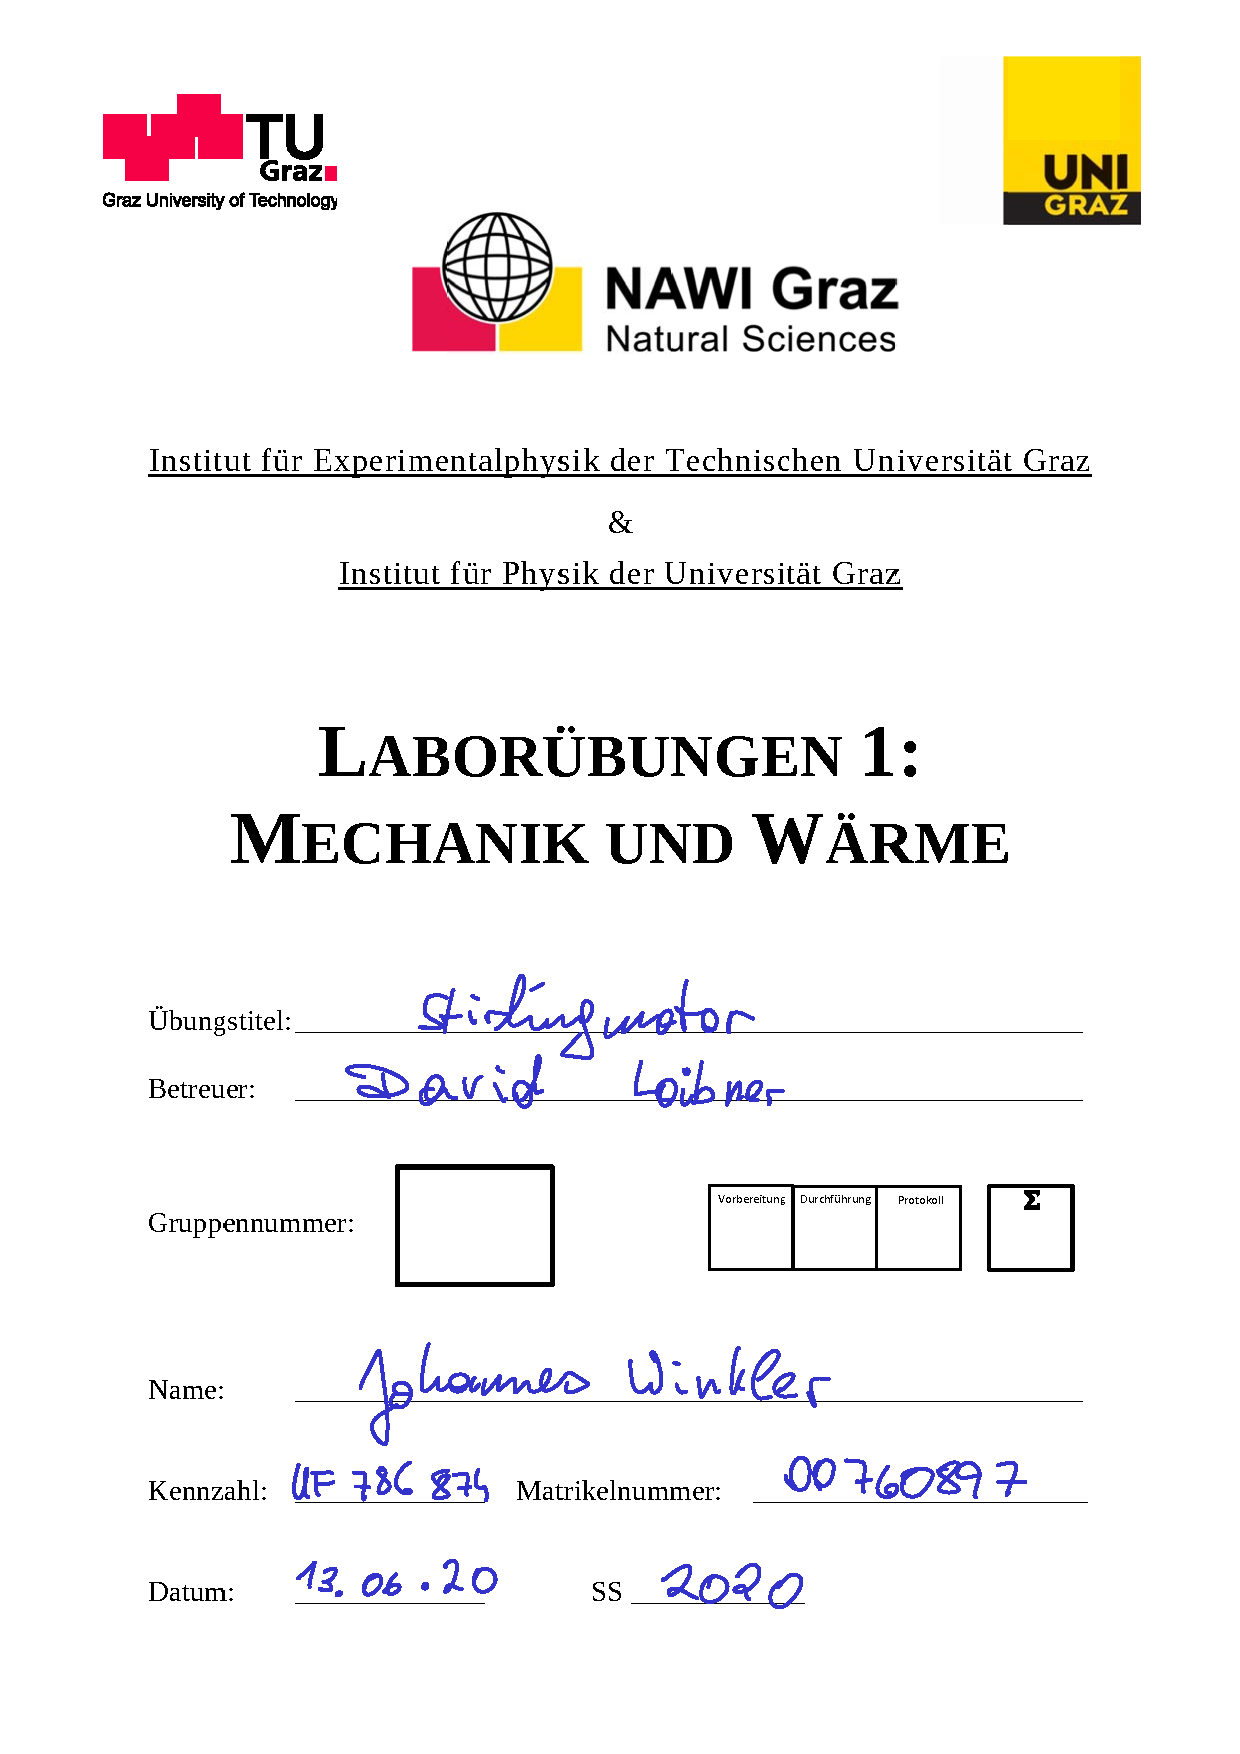
\includepdf[page=-]{deckblatt.pdf} 
 
 
\pagestyle{fancy}


\tableofcontents

\newpage


\section{Aufgabenstellung}

Es sind die Daten eines belasteten und unbelasteten Stirlingmotor auszuwerten. Folgende Dinge sind für beide Fälle zu berechnen:
\begin{enumerate}
\item pV-Diagramm und geleistete Arbeit pro Zyklus
\item Die Zeit für einen vollen Zyklus und die aus dem pV-Diagramm resultierende Leistung
\item Den Wirkungsgrad anhand der zugeführten Heizleistung in Relation zur erbrachten Leistung im pV-Diagramm
\item Den Wirkungsgrad des Motors anhand der Kühlwassertemperatur vorher und nach dem Durchlaufen des Motors
\item Die Drehzahlen anhand der gegebenen Daten und anhand des Frequenzspektrums.
\end{enumerate}

Für den belasteten Stirlingmotor soll zusätzlich das geleistete Drehmoment in Relation zur zugeführten Heizleistung berechnet werden.

\section{Beschreibung der Versuchsanordnung}

Ein Stirling-Motor ist eine Wärmekraftmaschine, die dem Stirling-Kreisprozess folgt (vgl. \cite{demtr1}). Es gibt folgende 4 Takte. 
\begin{itemize}
\item 1 -- 2: Isotherme Expansion
\item 2 -- 3: Isochore Abkühlung
\item 3 -- 4: Isotherme Komprimierung
\item 4 -- 1: Isochore Erwärmung
\end{itemize}

Die isochoren Teile bestehen aus Erwärmung durch eine Wärmequelle (in unserem Fall eine Heizung) und einer Abkühlung (durch Kühlwasser). Idealerweise gilt $Q_2=Q_4$, sodass die Wärme verlustfrei zwischengespeichert wird und nicht verloren geht. Unter diesen Umständen wäre der Wirkungsgrad maximal und würde jenem des allgemeinen Carnot-Prozesses entsprechen. Die 4 Takte sind in Grafik \ref{fig:pV_skizze} skizziert.


\begin{figure}[H]
\caption{Kreisprozess eines Stirling-Motors (vgl. \cite{demtr1})}
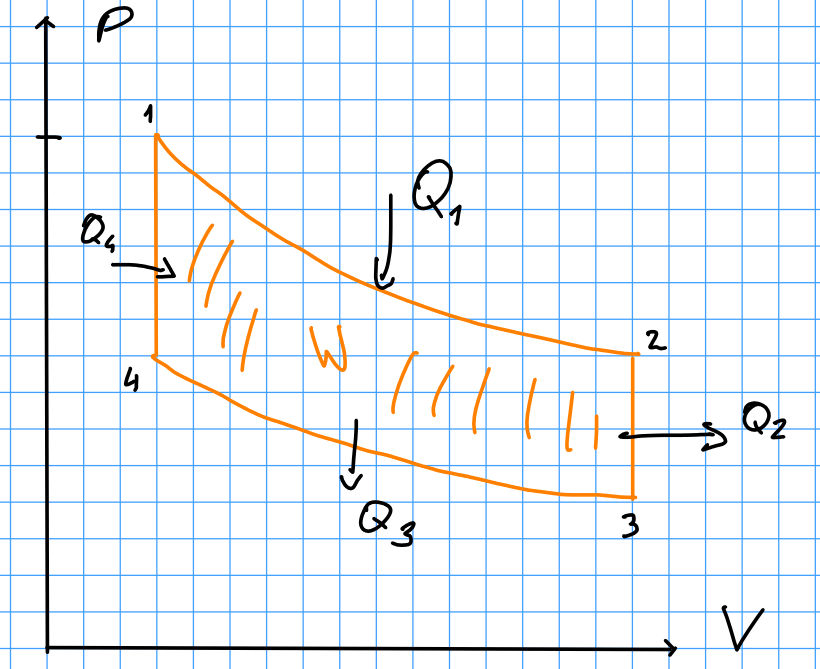
\includegraphics[height=7cm]{pV.png}
\label{fig:pV_skizze}
\end{figure}


Der Stirlingmotor arbeitet im Gegensatz zum Otto-Motor immer mit demselben Gas. Es gibt daher keine Ventile zum Ein- und Auslassen von Gas oder Gasgemischen.


Für die Bestimmung der geleisteten Arbeit ist eine numerische Integration erforderlich. Dafür wird die so genannten Gauss-Formel oder auch Shoelace-Formel verwendet. Diese findet man auf \cite{polygon}. Nachfolgend ist der dafür vorgesehene Python-Code.




\definecolor{commentgreen}{RGB}{2,112,10}
\definecolor{eminence}{RGB}{108,48,130}
\definecolor{weborange}{RGB}{255,165,0}
\definecolor{frenchplum}{RGB}{129,20,83}

\lstdefinelanguage{elixir}{
    morekeywords={def, for, range, abs, return},
    otherkeywords={<-,->, |>, \%\{, \}, \{, \, (, )},
    sensitive=true,
    morecomment=[l]{\#},
    morecomment=[n]{/*}{*/},
    morecomment=[s][\color{purple}]{:}{\ },
    morestring=[s][\color{orange}]"",
    commentstyle=\color{commentgreen},
    keywordstyle=\color{eminence},
    stringstyle=\color{red},
	basicstyle=\ttfamily,
	breaklines,
	showstringspaces=false,
	frame=tb
}

\begin{lstlisting}[language=elixir, caption={Gauss-Formel zur Berechnung der Fläche von Polygonen.},captionpos=b, label=lst:test]
def PolygonArea(x, y):
    A = 0.0
    n = len(x)
    for i in range(n):
        j = (i+1) % n
        A += x[i] * y[j]
        A -= x[j] * y[i]
    A = abs(A)/2
    return A
\end{lstlisting}

\section{Versuchsaufbauten}

Der Stirlingmotor wird einmal unbelastet und einmal belastet betrieben. Als Belastung wird ein Holzstab an der Drehscheibe befestigt, welches mit Reibung die Bewegung des Motors abbremst und ihn so belastet.

Die Messung des aktuellen Standes des Kolbens wird mit einem Drehwinkelaufnehmer gemessen. Aus diesem lässt sich neben der Position des Kolbens auch das Volumen berechnen.

Der Druck wird mit einem Schlauch an einen Druckaufnehmer weitergeleitet, wo der Druck dann elektronisch gemessen und gespeichert wird. Die Daten wie Druck, Volumen, Frequenz und Zeit werden in jeweils zwei csv-Dateien für den belasteten und unbelasteten Fall bereitgestellt.

\newpage

\section{Geräteliste}


Da aufgrund der Corona-Situation keine physikalische Anwesenheit im Labor möglich ist, kann ich auch die genauen Serien- und Gerätenummern angeben.

Da auch die Gebrauchsanleitung und Datenblätter mancher Werkzeuge nicht vorhanden sind, werden die Messfehler dieser Geräte geschätzt. Bei anderen wird die Unsicherheit im Video angegeben.


\begin{table}[h]
\caption{Geräteliste}

\begin{tabular}{lll}
Gerät  & Gerätenummer \\
\hline
Stirlingmotor & axxxx \\
Alkoholthermometer ($\Delta T = 0.25~^\circ$C) & bxxxx \\
Drehwinkelaufnehmer & cxxxx \\
Druckaufnehmer & dxxxx \\
Feder & exxxx \\
Federwaage ($\Delta F = 0.05~$N) & fxxxx \\
Maßband ($\Delta \ell = 1~$mm) & gxxxx\\
Messbecher ($\Delta V = 1.5~$ml) & hxxxx\\
Lenovo T430s (inkl. Ubuntu 18.04 und Python 3.6) & ixxxx\\
Stoppuhr ($\Delta t = 0.1~$s) & jxxxx \\
QPX1200L & kxxx
\end{tabular}
\end{table}

\newpage
\section{Versuchsdurchführung und Messergebnisse}

Die Temperaturen der Kühlflüssigkeiten werden zum Zwecke der Übersicht für belastet und unbelasteten Motor gemeinsam in Tabelle \ref{tab:kuehltemp} festgehalten.

\begin{table}[H]
\caption{Gemessene Temperaturen des Kühlwassers vor und nach dem Durchgang durch den Motor gemessen in Grad Celsius mit einer Abweichung von $\Delta T = 0.25~^\circ$C.}
\label{tab:kuehltemp}
\begin{tabular}{ccc|ccc}
\multicolumn{3}{c|}{unbelastet} & \multicolumn{3}{c}{belastet} \\
vorher & nachher & $T_\text{un}$ & vorher & nachher & $T_\text{be}$ \\
\hline
18.1 & 23.1 & 5.0 & 18.4 & 24.5 & 6.1
\end{tabular}
\end{table}

Die Durchflussmenge beim unbelasteten Motor geht im Video von 12:58 bei 30~ml bis 13:47 bei 230~ml. Das sind 49 Sekunden für 200~ml. Analog gilt für den belasteten Motor, dass die Durchflussmenge zwischen 16:29 und 17:18 gemessen wird. Die Füllmenge im Behälter ist wieder 30 bzw. 230~ml. Daher kann man in beiden Fälen eine Durchflussrate von 200~ml pro 49 Sekunden annehmen.

Zusammenfassend lässt sich sagen, dass $V_\text{W} = 200~$ml in $t_\text{W} = 49~$s fließen.

In der Praxis rechnet man das auf 
\begin{align}
\label{eq:menge}
\text{Durchflussmenge}~\frac{V_\text{W}}{t_\text{W}} = 4.0816~\text{ml pro Sekunde}
\end{align}


Die Heizleistungen lassen sich unkompliziert vom Gerät ablesen. Diese sind in Tabelle \ref{tab:heizleistung} dargestellt. Für die Heizleistung des belasteten Motors schwankt der Wert zwischen 249.1 und 249.2. Deshalb wird der Mittelwert dieser Werte angenommen.

\begin{table}[H]
\caption{Heizleistung für unbelasteten und belasteten Stirlingmotor in VA.}
\label{tab:heizleistung}
\begin{tabular}{c|c}
Heizleistung unbelastet / VA & Heizleistung unbelastet / VA \\
\hline
107.50 & 249.15

\end{tabular}
\end{table}

Zusätzlich kann man beim belasteten Motor noch die Kraft ablesen, die das Bremsholz auf eine Federwaage auswirkt und das daraus resultierende Drehmoment bestimmen. Der Hebelarm zwischen Antriebswelle und Federwaage sind $\ell=25~$cm entfernt. Zusätzlich lässt sich auf der Federwaage eine Kraft von 0.55~N messen.


Schließlich wurde Druck und Volumen im Motor sowohl im unbelasteten als auch im belastetem Zustand gemessen. Die daraus erhaltenen Messwerte liegen in csv-Dateien vor. Die Werte sind in den Grafiken \ref{fig:unbelastet_timeseries} und \ref{fig:belastet_timeseries} visualisiert.



\begin{figure}[H]
\caption{Unbelasteter Stirlingmotor.}
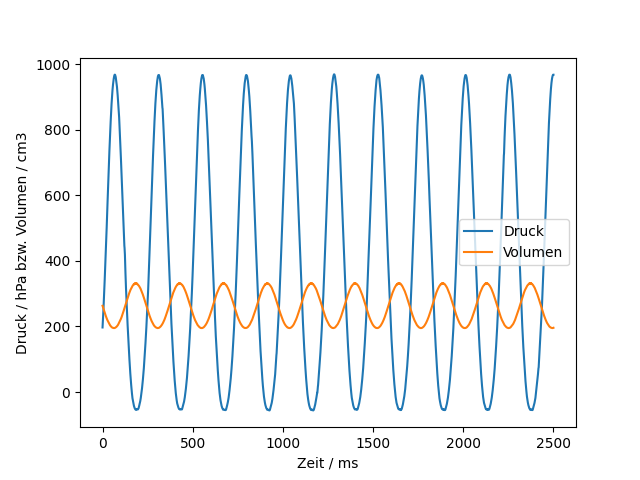
\includegraphics[height=7cm]{graphics/graphs_unbelastet.png}
\label{fig:unbelastet_timeseries}
\end{figure}


\begin{figure}[H]
\caption{Belasteter Stirlingmotor.}
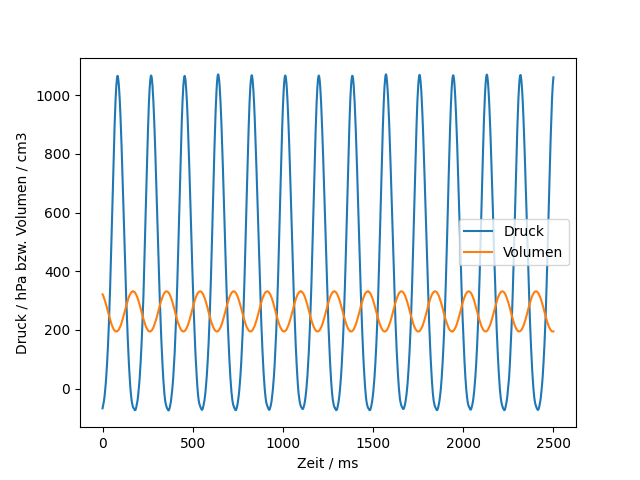
\includegraphics[height=7cm]{graphics/graphs_belastet.png}
\label{fig:belastet_timeseries}
\end{figure}


\newpage


\section{Auswertung}


\subsection{pV-Diagramme und Arbeit pro Zyklus}

Die pV-Diagramme sind in Abbildung \ref{fig:pV_orig} zu sehen. Die Fläche im pV-Diagramm (also die geleistete Arbeit) des unbelasteten Motors ist logischerweise kleiner als jene beim belasteten Motor. Das liegt daran, dass beim unbelasteten Motor nur die innere Reibung selbst als Arbeit verrichtet wird. Beim belasteten Motor kommt zusätzlich die geleistete mechanische Arbeit dazu.


\begin{figure}[H]
\caption{pV-Diagramme aus den gegebenen Daten zum Stirling-Motor.  }
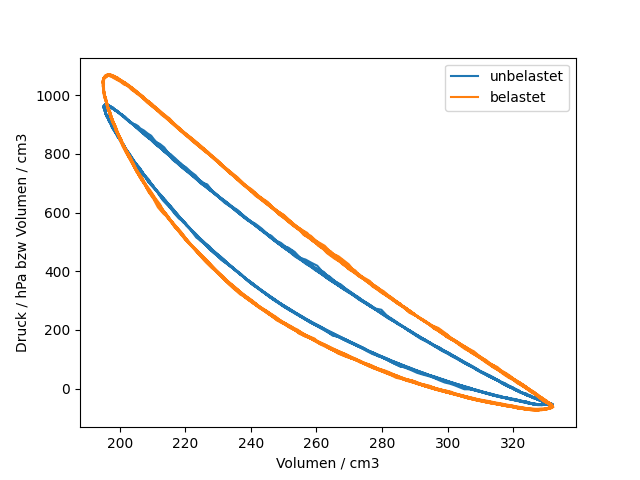
\includegraphics[height=7cm]{graphics/pV.png}
\label{fig:pV_orig}
\end{figure}


Die Arbeit pro Zyklus ist in Tabelle \ref{tab:arbeit_pro_zykl} dargestellt. Die Werte wurden mit Hilfe von \cite{skript} berechnet. Für die numerische Integration wurde der Code aus Listing \ref{lst:test} verwendet. 
\begin{table}[H]
\caption{Geleistete Arbeit pro Arbeitszyklus, berechnet durch numerische Integration der gegebenen Daten.}
\label{tab:arbeit_pro_zykl}
\begin{tabular}{l|ll}
Zyklus Nr. & unbelastet / J & belastet / J \\
\hline
1 & 1.8469 & 3.5436 \\
2 & 1.8838 & 3.5518 \\
3 & 1.8452 & 3.5174 \\
4 & 1.8983 & 3.6182 \\
5 & 1.8708 & 3.5938 \\
6 & 1.8695 & 3.5542 \\
7 & 1.9027 & 3.559 \\
8 & 1.8915 & 3.5184 \\
9 & 1.8833 & 3.5468 \\
10 &  & 3.5809 \\
11 &  & 3.564 \\
12 &  & 3.583 \\
\hline
Mittelwert & 1.8769 & 3.5609 \\
Spannweite & 0.0575 & 0.1009
\end{tabular}
\end{table}


\subsection{Drehzahl und abgegebene Leistung}

Nun müssen aus den Daten die mittlere Schwingungsdauer $t$ schätzen. Dies wird wieder mit Hilfe von \cite{skript} erledigt. Die Ergebnisse sind in Tabelle \ref{tab:cycl_length} sichtbar. Für die Berechnung der Dauer wurde die gesamte Zeitreihe verwendet und die Zyklenlängen entsprechend gemittelt. Dadurch wird das Ergebnis genauer und die Abweichung kleiner.
\begin{table}[H]
\caption{Längen eines Zyklus im pV Diagramm in Milisekunden}
\label{tab:cycl_length}
\begin{tabular}{l|ll}
Zyklus Nr. & unbelastet / ms & belastet / ms \\
\hline 
1 & 243 & 186 \\
2 & 242 & 186 \\
3 & 244 & 186 \\
4 & 244 & 186 \\
5 & 243 & 185 \\
6 & 243 & 187 \\
7 & 243 & 185 \\
8 & 243 & 187 \\
9 & 243 & 186 \\
10 &  & 187 \\
11 &  & 186 \\
12 &  & 187 \\
\hline
Mittelwert: & 243 & 186 \\
Spannweite: & 2 & 2 
\end{tabular}
\end{table}

Die Leistung berechnet sich aus dem Quotienten Arbeit pro Zeit. Also
\begin{align}
P = \frac{W}{\tau} = \begin{cases} \frac{1.8769 \text{J}}{0.2431 \text{s}} = 7.72 \text{W} & \text{ für unbelastet} \\ \frac{3.5609 \text{J}}{0.1862 \text{s}} = 19.12 \text{W} & \text{ für unbelastet} \\\end{cases}
\end{align}

Für die Unsicherheit der Leistung ergibt sich
\begin{align}
\Delta P &= \left|\frac{\partial P}{\partial W}\right| \cdot \Delta W + \left|\frac{\partial P}{\partial \tau}\right| \cdot \Delta \tau \\
\Delta P &= \frac{\Delta W}{\tau} + \frac{W}{\tau^2}\cdot \Delta \tau
\end{align}
Insgesamt ist die Leistung des Stirlingmotors daher
\begin{align*}
P_{\text{unbelastet}} &= (7.72 \pm 0.30)~\text{W} \\P_{\text{belastet}} &= (19.12 \pm 0.75)~\text{W} 
\end{align*}



\subsection{Zugeführte Energie beim Heizen}

Der Motor wird elektrisch mit Hilfe des Gerätes QPX1200L beheizt. Eine kurze Recherche im Internet ergibt laut \cite{heizung} eine Unsicherheit von $0.5~\%,~ \pm0.1~$W. Zusätzlich steht im Datenblatt, dass die maximale Auflösung 0.1~W ist.


Gemäß Tabelle \ref{tab:heizleistung} ergibt sich nun für die zugeführte Wärmeleistung
\begin{align*}
P_{Q,\text{unbelastet}} &= (107.50 \pm 0.70)~\text{W} \\
P_{Q,\text{unbelastet}} &= (249.15 \pm 1.40	)~\text{W}
\end{align*}



\subsection{Energiebilanz im Kühlwasser}

Für die Leistung die pro Zeiteinheit im Wasser abtransportiert wird, gilt
\begin{align}
P_\text{W} &= \frac{m_\text{W} \cdot c_\text{W} \cdot T}{ t_\text{W}} \\
&= \frac{\rho_\text{W} \cdot V_\text{W} \cdot c_\text{W} \cdot T}{ t_\text{W}} \\
&= \rho_\text{W}  \cdot c_\text{W} \cdot T\cdot\frac{ V_\text{W}}{ t_\text{W}}
\end{align}
wobei $\rho_\text{W} = 998~$kg/m${}^3$ (vgl. \cite{wasser_dichte}) die Dichte bei $20~^\circ$C und $c_\text{W} = 4186~\text{J/(kg K)}$ die Wärmekapazität (vgl. \cite{giancoli}) des Wassers ist. Der Term $V_\text{W} / t_\text{W}$ ist die Durchflussmenge pro Zeit. Diese wurde in \eqref{eq:menge} auf ca. 4~ml pro Sekunde bestimmt. Für die Unsicherheit gilt
\begin{align}
\Delta P_\text{W} &= \left| \frac{\partial P_\text{W}}{\partial T}\right| \cdot \Delta T + \left| \frac{\partial P_\text{W}}{\partial V_\text{W}}\right| \cdot \Delta V_\text{W} + \left| \frac{\partial P_\text{W}}{\partial t_\text{W}}\right| \cdot \Delta t_\text{W} \\
&= \rho_\text{W} \cdot c_\text{W} \cdot \left( \Delta T \cdot \frac{V_\text{W}}{t_\text{W}} + T\cdot \frac{\Delta V_\text{W}}{t_\text{W}} + T\cdot \frac{V_\text{W}}{t_\text{W}^2}\cdot \Delta t_\text{W} \right)
\end{align}
Zusätzlich ist $\Delta V = 1.5~$ml, $\Delta t_\text{W} = 0.1~$s und $\Delta T_\text{W} = 0.25~^\circ$C gegeben.


Insgesamt gilt für die Wärmeleistung im Wasser
\begin{align*}
P_{\text{W},\text{unbelastet}} &= (85.26 \pm 5.08)~\text{W} \\
P_{\text{W},\text{belastet}} &= (104.01 \pm 5.26)~\text{W} 
\end{align*}



\subsection{Drehmoment}

Das vom Motor geleistete Drehmoment ist das Produkt von Kraft und Kraftarm. Für Drehmoment und dessen Unsicherheit gilt
\begin{align}
M &= F\cdot \ell \\
\Delta M &= \left| \frac{\partial M}{\partial F}\right| \cdot \Delta F + \left| \frac{\partial M}{\partial \ell}\right| \cdot \Delta \ell \\
&= \Delta F \cdot \ell + F \cdot \Delta \ell
\end{align}
Zusätzlich ist $\Delta F = 0.05$~N und $\Delta r  = 1~$mm. Daraus folgt für das Drehmoment
\begin{align*}
M = (0.13750 \pm 0.01305)~\text{Nm}
\end{align*}

Die durch das Drehmoment abgegebene Leistung ist definiert als $P_\text{mech} = M \cdot \omega$, wobei $\omega$ die Winkelgeschwindigkeit ist. Es gilt also

\begin{align}
P_\text{mech} &= F\cdot \ell \cdot \omega = F\cdot \ell \cdot \frac{2\cdot\pi}{\tau} \\
\Delta P_\text{mech} &= \left| \frac{\partial P_\text{mech}}{\partial F}\right|\cdot\Delta F + \left| \frac{\partial P_\text{mech}}{\partial \ell}\right|\cdot\Delta \ell + \left| \frac{\partial P_\text{mech}}{\partial \tau}\right|\cdot\Delta \tau \\
&= 2\cdot \pi\cdot \left( \frac{\Delta F \cdot \ell + F\cdot \Delta \ell}{\tau} +  \frac{F\cdot \ell}{\tau^2}\cdot\Delta\tau\right)
\end{align}
Die Unsicherheit $\Delta \tau=2~$ms. Diese Berechnung gilt natürlich nur für den belasteten Stirlingmotor, da am unbelasteten kein Drehmoment abgegeben wird.

Insgesamt gilt für die mechanische Leistung, die in Form eines Drehmomentes abgegben wird
\begin{align*}
P_\text{mech} &= (4.64 \pm 0.08)~\text{W}
\end{align*}


\subsection{Wirkungsgrad}

Für die Berechnung des  Wirkungsgrades muss die gewonnene mechanische Energie (Leistung) mit der aufgewendeten Energie (Leistung) in Verhältnis gesetzt werden. Allgemein gilt
\begin{align}
\eta_L &= \frac{P_\text{out}}{P_\text{in}} \\
\Delta \eta_L &= \left| \frac{\partial\eta_L}{\partial P_\text{out}} \right| \cdot \Delta P_\text{out} + \left| \frac{\partial\eta_L}{\partial P_\text{in}} \right| \cdot \Delta P_\text{in} \label{eq:wirk_1}\\
&= \frac{\Delta P_\text{out}}{ P_\text{in}} + \frac{P_\text{out}}{P^2_\text{in}}\cdot \Delta P_\text{in}\label{eq:wirk_2}
\end{align}
Für den unbelasteten Motor gilt
\begin{align*}
\eta_L &\approx 7.18\% \\
\Delta \eta_L &\approx 3.25\%
\end{align*}

Für den belasteten Motor gilt
\begin{align*}
\eta_L &\approx 7.67\% \\
\Delta \eta_L &\approx 0.34\%
\end{align*}

Für den belasteten Stirlingmotor könnte man zusätzlich noch die am Drehmoment erbrachte Leistung zur gesamten investierten Leistung setzen.
Es ergibt sich daher
\begin{align*}
\eta_\text{mech} = \frac{P_\text{mech}}{P_\text{in}} = \frac{4.64}{249.15} = 1.86\%
\end{align*}
Dieser Wirkungsgrad ist sehr gering. Im Gegensatz zu $\eta_L$ zählt hier auch die innere Reibung als Verlustleistung, daher ist $\eta_\text{mech} < \eta_L$. Die Unsicherheit $\Delta_\text{mech} = 0.04\%$ erhalten wir hier analog zu Gleichungen \eqref{eq:wirk_1} und \eqref{eq:wirk_2}



\newpage
\section{Zusammenfassung}


Zusammenfassend ergeben sich folgende Werte 
\begin{table}[H]
\caption{Zusammenfassung aller charakteristischen Werte für den Motor}
\begin{tabular}{l|rr}
 & unbelastet & belastet \\
 \hline
Kühlwassertemp. vorher & ($18.1\pm 0.25)~{}^\circ$C & ($18.4\pm 0.25)~{}^\circ$C \\
Kühlwassertemp. nachher& ($23.1\pm 0.25)~{}^\circ$C & ($24.5\pm0.25)~{}^\circ$C \\
Drehzahl & $(4.11 \pm 0.5)~$s${}^{-1}$ & $(5.95 \pm 0.5)~$s${}^{-1}$ \\
Zugeführte Heizleistung & $(107.50 \pm 0.70)~$W & $(249.15 \pm 1.40)~$W \\
Abgeführte Leistung (Kühlmittel) & $(85.26 \pm 5.08)~$W & $(104.01 \pm 5.26)~$W\\
Arbeit nach pV-Diagramm & $(1.88 \pm 0.06)~$J & $(3.56 \pm 0.11)~$J \\
Gesamtleistung & $(7.72 \pm 0.30)~$W & $(19.12 \pm 0.75)~$W \\
Leistung (Drehmoment) & 0~W & $(4.64\pm 0.08)~$W \\
\hline
$\eta_L$ & $(7.18 \pm 3.35)\%$ & $(7.67 \pm 0.34)\%$ \\
$\eta_\text{mech}$ & -- & $(1.86 \pm 0.04)\%$
\end{tabular}
\end{table}

\section{Diskussion}

In den pV-Diagrammen in Grafik \ref{fig:pV_orig} sieht man, dass diese nur näherungsweise der theoretischen Vorlage in Grafik \ref{fig:pV_skizze} entsprechen. Das ist damit zu erklären, dass es in der Praxis immer Reibungseffekte gibt oder dass der Kolben nicht ganz dich ist, die nicht vom Modell berücksichtigt werden.

Wenn man die Differenz aus zugeführter und abgeführter Leistung berechnet, müsste man bei einem idealen Motor auf dasselbe Ergebnis für die Leistung kommen. Dies ist aber in der Praxis nicht möglich, da die erbrachte Heizleistung auch die Umgebung (Luft) und Teile vom Motor erwärmt. Hier würde es das der Messgenauigkeit scheitern. Für den unbelasteten Motor würde sich $1- 85.26/107.50 \approx 20\%$ ergeben, was deutlich mehr ist, als die erreichten $7\%$. Für den belasteten Motor wären es $1- 104.01/249.15 \approx 58\%$. Auch das wäre absurd hoch, hier weicht der Wert sogar noch stärker ab, da bei hoher Heizleistung mehr Wärme in andere Richtung abstrahlt. Daher ist die andere Methode zur Berechnung sinnvoller, da dort die abgestrahlte Verlustwärme nicht extra berücksichtigt werden muss.


Die Dauer eines Zyklus (bzw. die Frequenz) hätte man stattdessen auch durch eine Fouriertransformation berechnen können. Das sieht man in Grafik \ref{fig:fourier}. Die Schwigungsdauer eines unbelasteten Motors ist bei ca. 243~ms, was einer Frequenz von 4.12~Hz entspricht. Analog sind es 5.38~Hz für den belasteten Stirlingmotor. 


\begin{figure}[H]
\caption{Frequenzspektrum.}
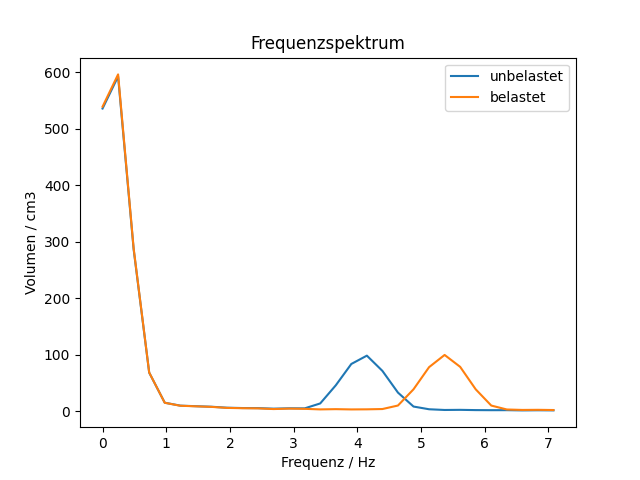
\includegraphics[height=7cm]{graphics/freq.png}
\label{fig:fourier}
\end{figure}



\begin{thebibliography}{9}
\bibitem{demtr1} W. Demtröder, \emph{Experimentalphysik 1: Mechanik und Wärme}, Springer-Spektrum, 8. Auflage, 2018.

\bibitem{giancoli} D. Giancoli, \emph{Physik}, Pearson, 4. Auflage, 2019.

\bibitem{skript} J. Winkler, \url{https://github.com/jowin202/lab_tugraz/blob/master/numeric.py} (Stand: \today)

\bibitem{wasser_dichte} \url{https://www.internetchemie.info/chemie-lexikon/daten/w/wasser-dichtetabelle.php} (Stand: \today)


\bibitem{polygon} \url{https://en.wikipedia.org/wiki/Shoelace_formula} (Stand: \today)

\bibitem{heizung} \url{https://www.aimtti.com/product-category/dc-power-supplies/aim-qpxseries} (Stand: \today)


\end{thebibliography}

\end{document}
